\documentclass[12pt,a4paper]{article}
\usepackage[UTF8]{ctex}
\usepackage{amsmath}
\usepackage{graphicx}
\usepackage{booktabs}
\usepackage{geometry}
\usepackage{pgfplots}
\pgfplotsset{compat=1.17}
\usepackage{ulem}
\geometry{left=2.5cm,right=2.5cm,top=2.5cm,bottom=2.5cm}

\title{\Huge{\textbf{\uuline{凯\ 特\ 摆\ 实\ 验\ 报\ 告}}}}
% 按照“衍射实验报告.tex”的格式样式设置作者栏；如需修改请直接编辑下行信息。
\author{\uline{少年班学院} \quad 姓名: \uline{徐子钦} \quad 学号: \uline{PB24000224}}
\date{\today}

\begin{document}
\maketitle

\begin{abstract}
本实验利用凯特摆测量当地重力加速度。通过测量凯特摆在正挂和倒挂两种状态下的摆动周期，以及两刀口之间的距离，利用贝塞尔公式计算重力加速度。实验测得当地重力加速度为 $g = 9.809 \pm 0.017 \,\text{m/s}^2$，与参考值相比相对误差约为 $0.16\%$。结果表明，凯特摆法能够有效消除转动惯量和重心位置测量带来的误差，是一种高精度的重力加速度测量方法。
\end{abstract}

\section{实验目的}
\begin{enumerate}
    \item 了解凯特摆的结构和原理。
    \item 掌握用凯特摆精确测量重力加速度的方法。
    \item 学习利用贝塞尔公式处理数据，减小误差。
\end{enumerate}

\section{实验原理}
凯特摆是一种复摆。本实验保持凯特摆的质量分布不变（即不调节重物位置），分别以两个不对称的刀口为悬挂点，测量其摆动周期 $T_1$ 和 $T_2$。

设凯特摆绕质心的转动惯量为 $I_0$，质量为 $m$。根据刚体定轴转动定律，复摆绕悬点 $O$（距离质心 $h$）作微小摆动的周期 $T$ 为：
\[ T = 2\pi \sqrt{\frac{I}{mgh}} \]
根据平行轴定理 $I = I_0 + mh^2$，代入上式得：
\[ T = 2\pi \sqrt{\frac{I_0 + mh^2}{mgh}} = 2\pi \sqrt{\frac{\frac{I_0}{m} + h^2}{gh}} \]
令 $k^2 = I_0/m$（$k$ 为回转半径），则有：
\[ T^2 = \frac{4\pi^2}{g} \left( \frac{k^2}{h} + h \right) \quad \Rightarrow \quad \frac{gT^2}{4\pi^2} h = k^2 + h^2 \]

分别以两个刀口为悬点时，重心到刀口的距离分别为 $h_1$ 和 $h_2$，对应的周期为 $T_1$ 和 $T_2$。代入上式可得方程组：
\begin{equation}
    \frac{gT_1^2}{4\pi^2} h_1 = k^2 + h_1^2 
\end{equation}
\begin{equation}
    \frac{gT_2^2}{4\pi^2} h_2 = k^2 + h_2^2
\end{equation}

消去未知量 $k^2$（(1)式减(2)式）：
\[ \frac{g}{4\pi^2} (T_1^2 h_1 - T_2^2 h_2) = h_1^2 - h_2^2 \]
整理得重力加速度 $g$ 的表达式：
\[ g = \frac{4\pi^2 (h_1^2 - h_2^2)}{T_1^2 h_1 - T_2^2 h_2} \]

为了减少 $h_1, h_2$ 测量误差的影响，通常将其改写为贝塞尔公式的形式。利用恒等变换：
\[ \frac{T_1^2 h_1 - T_2^2 h_2}{h_1^2 - h_2^2} = \frac{(T_1^2 + T_2^2)(h_1 - h_2) + (T_1^2 - T_2^2)(h_1 + h_2)}{2(h_1 - h_2)(h_1 + h_2)} = \frac{T_1^2 + T_2^2}{2(h_1 + h_2)} + \frac{T_1^2 - T_2^2}{2(h_1 - h_2)} \]
故重力加速度 $g$ 可由下式给出（贝塞尔公式）：
\[ \frac{4\pi^2}{g} = \frac{T_1^2 + T_2^2}{2(h_1 + h_2)} + \frac{T_1^2 - T_2^2}{2(h_1 - h_2)} \]

其中：
\begin{itemize}
    \item $T_1, T_2$ 分别为正挂和倒挂时的周期；
    \item $h_1, h_2$ 分别为重心到两个刀口的距离（$h_1$ 为正挂刀口到重心距离，$h_2$ 为倒挂刀口到重心距离）；
    \item $h_1 + h_2 = L$ 为两刀口之间的距离。
\end{itemize}
实验中直接测量两刀口间距 $L$ 以及其中一个刀口到重心的距离 $h_1$，则可求出 $h_2 = L - h_1$ 及 $h_1 - h_2 = 2h_1 - L$，代入公式即可求得 $g$。

\section{实验器材}
\begin{itemize}
    \item 凯特摆装置（固定质量分布）；
    \item 秒表或光电门计时器；
    \item 米尺（用于测量刀口间距及重心位置）；
    \item 支架与水平调节装置。
\end{itemize}

\section{实验步骤与方法}
\begin{enumerate}
    \item 调节底座水平，确保摆动平面垂直水平面。
    \item 测量两刀口之间的距离 $L$，重复测量 3 次取平均。
    \item 取下凯特摆，在刀口外寻找平衡位置确定重心，测量正挂刀口到重心的距离 $h_1$，重复测量 3 次取平均。
    \item 将凯特摆正挂（以刀口 1 悬挂），测量 10 个周期的总时间 $t_1$，重复测量多次取平均，计算周期 $T_1 = t_1/10$。
    \item 将凯特摆倒挂（以刀口 2 悬挂），测量 10 个周期的总时间 $t_2$，重复测量多次取平均，计算周期 $T_2 = t_2/10$。
    \item 利用贝塞尔公式计算重力加速度 $g$。
\end{enumerate}

\section{原始数据}
\subsection*{几何参数}
\begin{center}
\begin{tabular}{cccc}
	\toprule
    序号 & 两刀口间距 $L$ (m) & 正挂刀口到重心距离 $h_1$ (m) & 倒挂刀口到重心距离 $h_2$ (m) \\
    \midrule
	1 & 0.7510 & 0.4420 & 0.3090 \\
	2 & 0.7500 & 0.4480 & 0.3020 \\
	3 & 0.7510 & 0.4460 & 0.3050 \\
    \midrule
    平均值 & $\bar{L} = 0.7507$ & $\bar{h}_1 = 0.4453$ & $\bar{h}_2 = 0.3054$ \\
    \bottomrule
\end{tabular}
\end{center}
\subsection*{周期测量数据 (10个周期时间)}
\begin{center}
\begin{tabular}{ccc}
\toprule
序号 & 正挂 10$T_1$ (s) & 倒挂 10$T_2$ (s) \\
\midrule
1  & 17.3862 & 17.3905 \\
2  & 17.3862 & 17.3882 \\
3  & 17.3876 & 17.3877 \\
4  & 17.3873 & 17.3892 \\
5  & 17.3865 & 17.3889 \\
\midrule
平均值 & $\bar{t}_1 = 17.3868$ & $\bar{t}_2 = 17.3889$ \\
周期 & $T_1 = 1.73868$ & $T_2 = 1.73889$ \\
\bottomrule
\end{tabular}
\end{center}


\section{数据处理与计算}
\subsection*{参数计算}
\begin{itemize}
    \item 两刀口间距：$L = 0.7507 \text{m}$
    \item 重心位置参数：$h_1 = 0.4453 \text{m}, \quad h_2 = L - h_1 = 0.3054 \text{m}$
    \item 几何项：$h_1 + h_2 = L = 0.7507 \text{m}, \quad h_1 - h_2 = 0.1400 \text{m}$
    \item 周期：$T_1 = 1.73868 \text{s}, \quad T_2 = 1.73889 \text{s}$
\end{itemize}

\subsection*{计算重力加速度 $g$}
代入贝塞尔公式：
\[ \frac{4\pi^2}{g} = \frac{T_1^2 + T_2^2}{2L} + \frac{T_1^2 - T_2^2}{2(h_1 - h_2)} \]
计算各项数值：
\[ A = \frac{T_1^2 + T_2^2}{2L} = \frac{1.73868^2 + 1.73889^2}{2 \times 0.7507} \approx 4.0276 \]
\[ B = \frac{T_1^2 - T_2^2}{2(h_1 - h_2)} = \frac{1.73868^2 - 1.73889^2}{2 \times 0.1400} \approx -0.0027 \]
\[ g = \frac{4\pi^2}{A + B} = \frac{39.4784}{4.0276 - 0.0027} \approx 9.809 \text{m/s}^2 \]

\subsection*{不确定度计算}
根据贝塞尔公式，令 $Y = \frac{4\pi^2}{g} = \frac{T_1^2 + T_2^2}{2L} + \frac{T_1^2 - T_2^2}{2(h_1 - h_2)}$。
由于实验中调节使得 $T_1 \approx T_2$，公式中第二项（修正项）数值极小。更重要的是，该项对重心位置 $h_1, h_2$ 的偏导数含有因子 $(T_1^2 - T_2^2)$，也趋近于零。这意味着重心位置 $h_1, h_2$ 的测量误差对最终结果的影响被极大地抑制（这也正是凯特摆设计的精妙之处：消除重心位置测量不准带来的误差）。因此，在计算不确定度时，可以忽略第二项的贡献，仅考虑第一项 $Y_1 = \frac{T_1^2 + T_2^2}{2L}$ 引入的误差。

重力加速度的相对不确定度为：
\[ u_r(g) = u_r(Y) \approx u_r(Y_1) = \sqrt{ \left(\frac{u(L)}{L}\right)^2 + \frac{u(T_1^2 + T_2^2)^2}{(T_1^2 + T_2^2)^2} } \]
其中 $u(T_1^2 + T_2^2) = \sqrt{(2T_1 u(T_1))^2 + (2T_2 u(T_2))^2}$。
若近似认为 $T_1 \approx T_2 \approx T$，则公式可简化为：
\[ u_r(g) \approx \sqrt{ \left(\frac{u(L)}{L}\right)^2 + \frac{u(T_1)^2 + u(T_2)^2}{T^2} } \]

\noindent\textbf{分量计算：}
\begin{enumerate}
    \item $u(L)$：由 A 类不确定度（3次测量标准差）与 B 类不确定度（米尺，$\Delta_{\text{inst}}$）合成。
    \[ u(L) = \sqrt{S_{\bar{L}}^2 + u_B(L)^2} \]
    \item $u(T_1), u(T_2)$：$T = t/10$，故 $u(T) = u(t)/10$。$u(t)$ 由 A 类（多次测量标准差）与 B 类（计时器精度）合成。
\end{enumerate}

\noindent\textbf{计算结果：}
\[ u_r(g) \approx \frac{u(L)}{L} = \frac{0.0007}{0.7507} \approx 0.09\% \]
\[ U_g = k \cdot u_r(g) \cdot g = 1.96 \times 0.0009 \times 9.809 \approx 0.017 \,\text{m/s}^2 \quad (k=1.96, P=0.95) \]

\section{结果与讨论}
\subsection*{主要结果}
\begin{itemize}
    \item 测得当地重力加速度 $g = (9.809 \pm 0.017) \,\text{m/s}^2 \quad (P=0.95)$。
    \item 相对误差：$\frac{|9.809 - 9.793|}{9.793} \times 100\% \approx 0.16\%$（参考合肥重力加速度 $g_{\text{std}}=9.793\,\text{m/s}^2$）。
\end{itemize}

\subsection*{误差分析}
\begin{enumerate}
    \item 长度测量误差；
    \item 周期测量误差（计时器精度、摆动角度影响）；
    \item 空气阻力影响；
    \item 刀口磨损或底座不水平。
\end{enumerate}

\section{思考题}
\begin{enumerate}
    \item \textbf{凯特摆测量重力加速度，在实验设计上有什么特点？避免了什么量的测量？降低了哪个量测量精度？实验室如何来实现？} \\
    \textbf{特点：}利用复摆的可逆性原理，即当复摆绕两个不对称的轴摆动周期相等时，两轴间距等于等效单摆长。\\
    \textbf{避免的测量：}避免了对复摆转动惯量 $I$ 和质心位置（重心）的精确测量。\\
    \textbf{降低精度的量：}降低了对重心到刀口距离 $h_1, h_2$ 的测量精度要求。因为在 $T_1 \approx T_2$ 时，贝塞尔公式中包含 $h_1, h_2$ 的修正项数值很小，其误差对结果影响极小。\\
    \textbf{实现：}实验室通常通过调节摆杆上的重物位置（改变质量分布）使正倒挂周期趋于一致，或者如本实验采用固定质量分布，直接测量两周期并利用贝塞尔公式计算。

    \item \textbf{结合误差计算，影响凯特摆测量精度的主要因素是什么？将所得的实验结果与当地的重力加速度的公认值比较，有无偏差？为什么？} \\
    \textbf{主要因素：}长度 $L$（两刀口间距）的测量误差和周期 $T$ 的测量误差。由于 $g \propto L/T^2$，周期的相对误差影响较大，但长度测量往往受限于仪器（米尺）精度。此外，刀口磨损（非几何线接触）和底座不水平也会引入误差。\\
    \textbf{偏差分析：}通常测得值会略小于公认值。主要原因包括：(1) 空气浮力减小了有效重力；(2) 空气阻力使振动周期变大；(3) 摆角非零（大角度近似误差）导致周期偏大。

    \item \textbf{摆的角振幅的大小，对实验结果有无影响？} \\
    \textbf{有影响。}计算公式 $T=2\pi\sqrt{L/g}$ 基于单摆的小角度近似 ($\sin\theta \approx \theta$)。实际上周期随振幅 $\theta$ 增大而增大：$T = T_0 (1 + \frac{1}{4}\sin^2(\frac{\theta}{2}) + \dots)$。若角振幅过大，测得周期 $T$ 偏大，导致计算出的 $g$ 偏小。实验中应控制摆角在 $5^\circ$ 以内。

    \item \textbf{总结测量重力加速度的方法，比较其优缺点。} \\
    \textbf{单摆法：}原理简单，但受摆线质量、弹性及质心位置测量限制，精度较低。\\
    \textbf{凯特摆法：}利用刚体复摆原理，消除了转动惯量和质心测量的误差，长度 $L$ 可精确测量，精度高，是实验室测 $g$ 的经典精密方法。\\
    \textbf{自由落体法：}直接反映定义，但时间测量要求极高，且受空气阻力影响大。\\
    \textbf{重力仪法：}利用弹簧静力平衡原理，精度极高且便携，但设备昂贵，常用于相对重力测量。

    \item \textbf{为什么凯特摆设计成：较重；摆锤不同材质；摆锤大小不同；摆锤是圆形；重量不同形状不同的摆锤交叉安放？} \\
    \textbf{较重：}为了减小空气阻力和浮力对实验结果的相对影响，并保证摆动惯性大，衰减慢，利于长时间测量周期。\\
    \textbf{不同材质/大小/交叉安放：}主要是为了构造不对称的物理摆。通过大小不同的摆锤和非对称安放，可以大幅调节重心位置，确保正挂和倒挂时重心到刀口的距离 $h_1 \neq h_2$，满足复摆测量的物理条件。\\
    \textbf{圆形：}形状规则，空气阻力各向同性且较小，便于加工和定位。

    \item \textbf{讨论凯特摆测量结果是否准确，跟单摆相比哪个更精确？为什么会这样？} \\
    \textbf{凯特摆更精确。}单摆实验中，摆线有质量、不可伸长假设难满足，且小球并非质点，最关键的是“摆长”（悬点到球心）难以精确测量。凯特摆作为刚体，不需要质点假设，且通过贝塞尔公式巧妙消除了转动惯量和重心位置测量不准的影响，只需测量两刀口之间的固定距离 $L$（可用比长仪测得很准）和周期，因此精度远高于单摆。
\end{enumerate}

\appendix
\section{实验原始数据}
\begin{figure}[h]
    \centering
    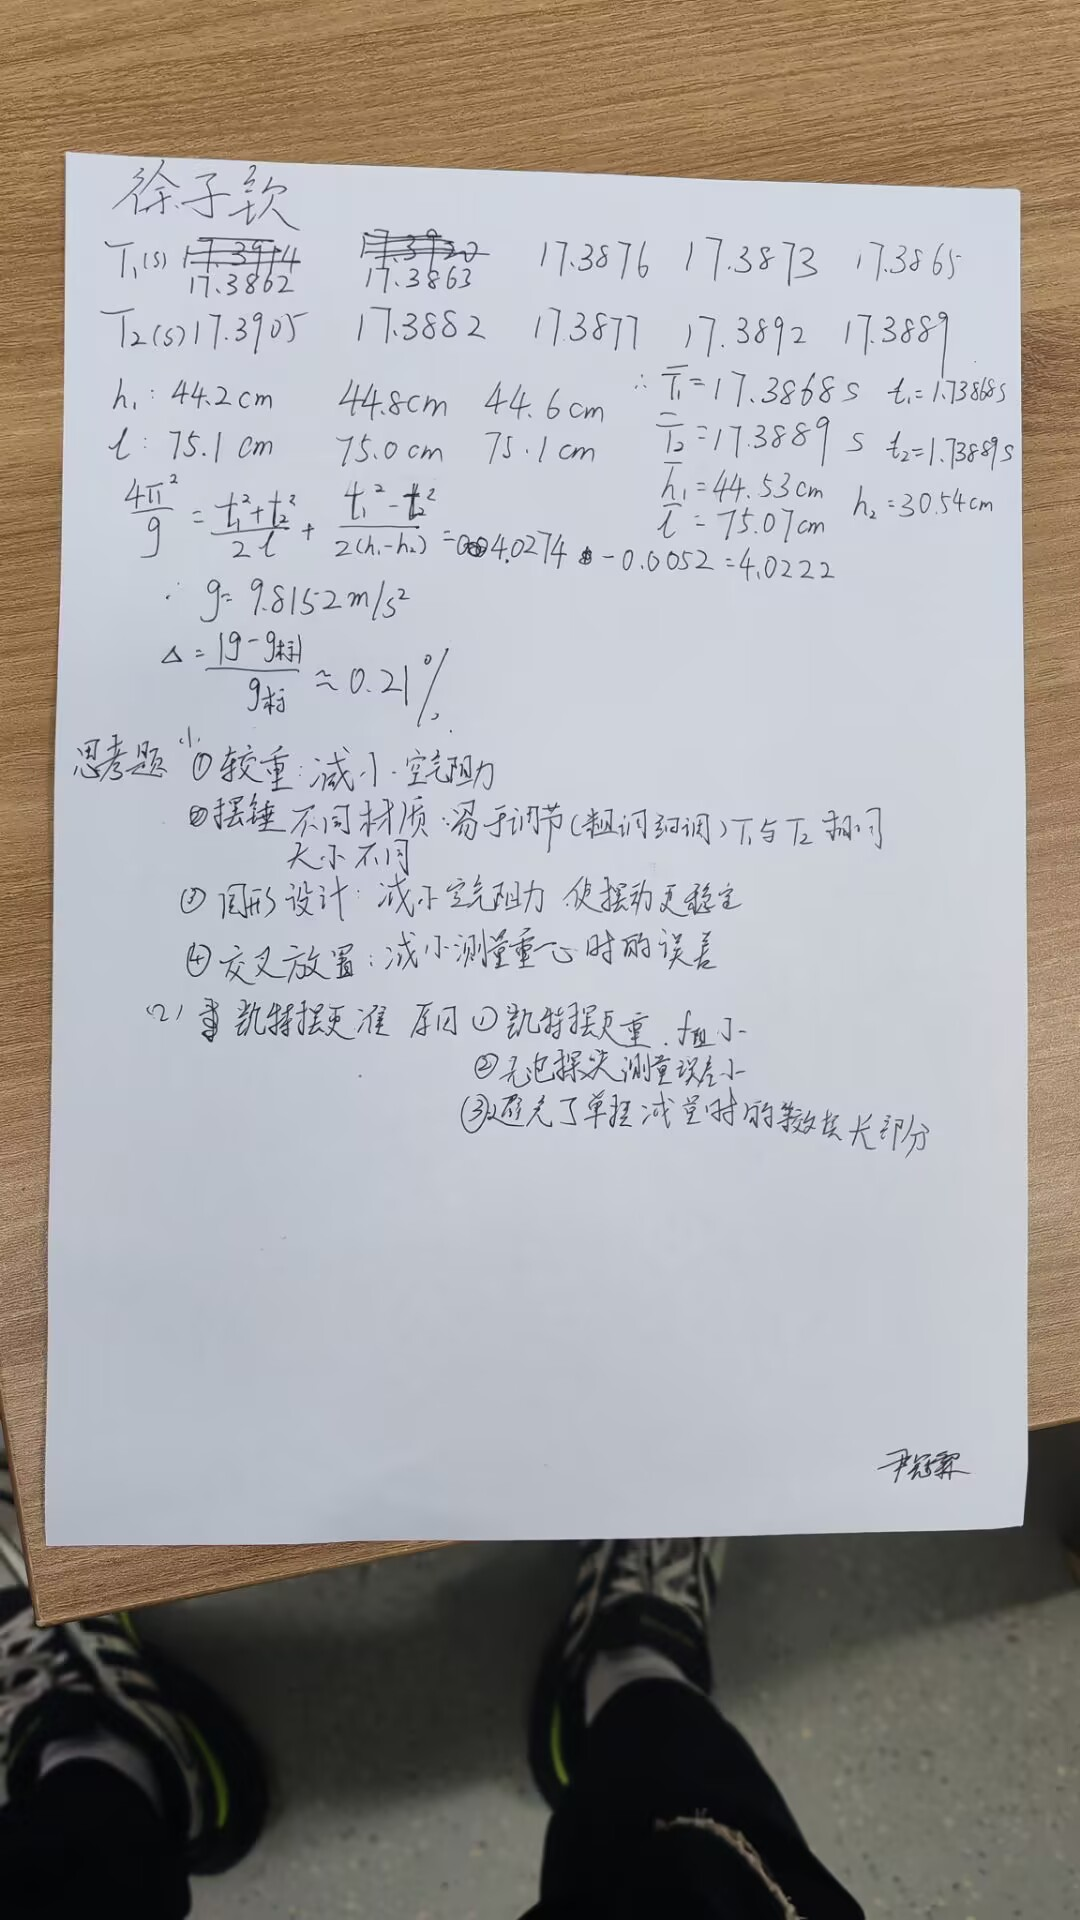
\includegraphics[width=0.6\textwidth]{原始数据.jpg}
    \caption{原始数据记录}
\end{figure}

\end{document}
